% !TEX options=--shell-escape
\documentclass [12pt]{article} 

\usepackage {amsmath}
\usepackage {amsthm}
\usepackage {amssymb}
\usepackage {graphicx} 
\usepackage {float}
\usepackage {multirow}
\usepackage {xcolor}
\usepackage {algorithmic}
\usepackage [ruled,vlined,commentsnumbered,titlenotnumbered]{algorithm2e} \usepackage {array} 
\usepackage {booktabs} 
\usepackage {url} 
\usepackage {parskip} 
\usepackage [margin=1in]{geometry} 
\usepackage [T1]{fontenc} 
\usepackage {cmbright} 
\usepackage [many]{tcolorbox} 
\usepackage [colorlinks = true,
            linkcolor = blue,
            urlcolor  = blue,
            citecolor = blue,
            anchorcolor = blue]{hyperref} 
\usepackage {enumitem} 
\usepackage {xparse} 
\usepackage {verbatim}
\usepackage{listings}
\usepackage{xcolor}
\usepackage{csquotes}
\usepackage[cache=false]{minted}
\usepackage{mdframed}
\newtheorem{theorem}{Theorem}

\BeforeBeginEnvironment{minted}{\begin{mdframed}}
\AfterEndEnvironment{minted}{\end{mdframed}}

\DeclareTColorBox {Solution}{}{breakable, title={Solution}}
\DeclareTColorBox {Solution*}{}{breakable, title={Solution (provided)}}
\DeclareTColorBox {Instruction}{}{boxrule=0pt, boxsep=0pt, left=0.5em, right=0.5em, top=0.5em, bottom=0.5em, arc=0pt, toprule=1pt, bottomrule=1pt}
\DeclareDocumentCommand {\Expecting }{+m}{\textbf {[We are expecting:} #1\textbf {]}}
\DeclareDocumentCommand {\Points }{m}{\textbf {(#1 pt.)}} 

\begin {document} 

{\LARGE \textbf {COMP 285 (NC A\&T, Spr `22)}\hfill \textbf {Homework 4} } 
\vspace {1em} 
\begin {Instruction} 

\paragraph {Due.} Wednesday, February 16th, 2022 @ 11:59 PM!
\end {Instruction} 

\vspace {1em} 
\begin {Instruction} \paragraph {Homework Expectations:} Please see \href{https://www.comp285.ml/homework/#general-homework-information}{Homework}.
\end {Instruction}

\vspace {1em} 
\begin {Instruction} 

\paragraph {Exercises} The following questions are exercises. We encourage you to work with a group and discuss solutions to make sure you understand the material.

\paragraph {Points} This assignment is graded out of 100 points. However, you can get up to 120 points if you complete everything. These are not bonus points, but rather points to help make-up any parts you miss.

\end {Instruction} 

\begin{centering}
\section*{Random Fun with Selection, Non-Comparions Sorts, and Data Structures}
\end{centering}

\begin{Instruction}

\paragraph{Written Problems} The following questions are to be submitted in written/typed form to gradescope.

\end{Instruction}

\section{Interview Practice: Modifying the Select Algorithm \Points{20}}

After class, Kevin, Tobiloba, and Hassan got together to discuss a few modifications to the `Select' algorithm we learned in class. Recall that in the `Select' algorithm, the runtime is represented with the recurrence:

\begin{align*}
T(n) = O(n) + T\left(\frac{n}{5}\right) + T\left(\frac{7n}{10}\right)
\end{align*}

Here, $T(\frac{n}{5})$ is for selecting the pivot, and $T(\frac{7n}{10})$ is for the recursive call to select the k-th element. If you need a refresher, see Lecture 8 (and maybe Lecture 7). 


\subsection{Bigger, Bigger, Bigger Chunks! \Points{10}}

Consider the modified version of the select algorithm, where we split our array into $\lceil \frac{n}{7}\rceil$ groups of size $\leq 7$ instead. What would be the recurrence relation for this modified version? What would be the running time?\footnote{You can't use the Master Theorem directly, but can you upper bound the recurrence? You can assume, for example, $T(n) = T(2n/5) + T(n/5) \leq T(3n/5)$.}

\Expecting{The recurrence relation for this modified algorithm as well as the running time in $O(\cdots)$ notation.}

\subsection{Smaller, Smaller, Smaller Chunks! \Points{10}}

Now consider another modified version of the select algorithm, where we split our array into $\lceil n/3 \rceil$ groups of size $\leq 3$ instead. What would be the recurrence relation for this modified version? What would be the running time.

\Expecting{The recurrence relation for this modified algorithm as well as the running time in $O(\cdots)$ notation.}


\pagebreak
\section{Exercise: Practice with Colors and Shakespeare \Points{10}}
Look at each of the following examples of trees. If you can color the nodes red or black to give a legitimate red-black tree (eg, it must follow our the rules discused in Lecture 12), then provide such a coloring. 

\subsection{To Tree or not to Tree, that is the question... \Points{5}}
\begin{center}
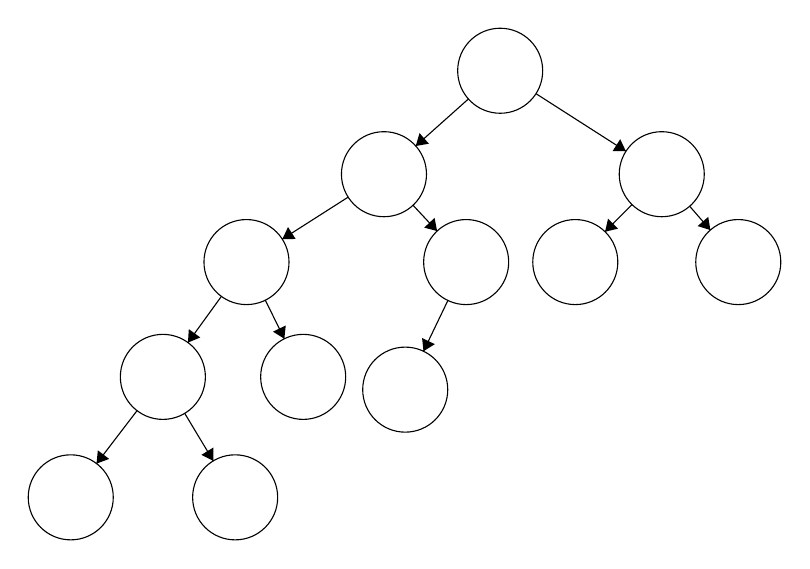
\begin{tikzpicture}[scale=0.18]
\tikzstyle{every node}+=[inner sep=0pt]
\draw [black] (39.9,-7.8) circle (3);
\draw [black] (31.7,-15.1) circle (3);
\draw [black] (51.3,-15.1) circle (3);
\draw [black] (56.7,-21.3) circle (3);
\draw [black] (45.2,-21.3) circle (3);
\draw [black] (37.5,-21.3) circle (3);
\draw [black] (22,-21.3) circle (3);
\draw [black] (33.2,-30.3) circle (3);
\draw [black] (26,-29.4) circle (3);
\draw [black] (16.1,-29.4) circle (3);
\draw [black] (21.2,-37.9) circle (3);
\draw [black] (9.6,-37.9) circle (3);
\draw [black] (37.66,-9.79) -- (33.94,-13.11);
\fill [black] (33.94,-13.11) -- (34.87,-12.95) -- (34.21,-12.2);
\draw [black] (33.75,-17.29) -- (35.45,-19.11);
\fill [black] (35.45,-19.11) -- (35.27,-18.18) -- (34.54,-18.87);
\draw [black] (42.43,-9.42) -- (48.77,-13.48);
\fill [black] (48.77,-13.48) -- (48.37,-12.63) -- (47.83,-13.47);
\draw [black] (49.2,-17.24) -- (47.3,-19.16);
\fill [black] (47.3,-19.16) -- (48.22,-18.94) -- (47.51,-18.24);
\draw [black] (53.27,-17.36) -- (54.73,-19.04);
\fill [black] (54.73,-19.04) -- (54.58,-18.11) -- (53.83,-18.76);
\draw [black] (36.21,-24.01) -- (34.49,-27.59);
\fill [black] (34.49,-27.59) -- (35.29,-27.09) -- (34.39,-26.66);
\draw [black] (23.33,-23.99) -- (24.67,-26.71);
\fill [black] (24.67,-26.71) -- (24.77,-25.77) -- (23.87,-26.21);
\draw [black] (20.23,-23.72) -- (17.87,-26.98);
\fill [black] (17.87,-26.98) -- (18.74,-26.62) -- (17.93,-26.03);
\draw [black] (29.17,-16.72) -- (24.53,-19.68);
\fill [black] (24.53,-19.68) -- (25.47,-19.67) -- (24.93,-18.83);
\draw [black] (14.28,-31.78) -- (11.42,-35.52);
\fill [black] (11.42,-35.52) -- (12.31,-35.19) -- (11.51,-34.58);
\draw [black] (17.64,-31.97) -- (19.66,-35.33);
\fill [black] (19.66,-35.33) -- (19.67,-34.38) -- (18.82,-34.9);
\end{tikzpicture}
\end{center}

\Expecting{Either an image of a colored-in red-black tree or a statement that "No such red-black tree exists." No need to justify your answer.}

\subsection{What's in a tree? That which we call a node, by any other word would color just as well... \Points{5}}

\begin{center}
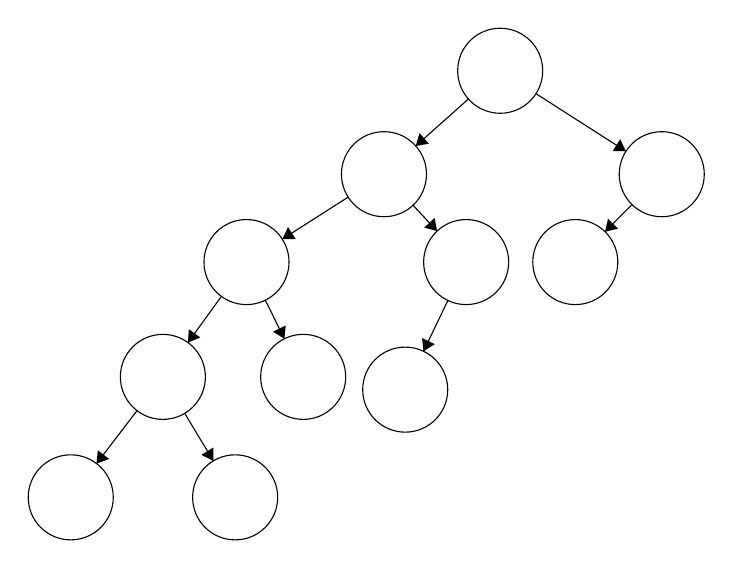
\begin{tikzpicture}[scale=0.18]
\tikzstyle{every node}+=[inner sep=0pt]
\draw [black] (39.9,-7.8) circle (3);
\draw [black] (31.7,-15.1) circle (3);
\draw [black] (51.3,-15.1) circle (3);
\draw [black] (45.2,-21.3) circle (3);
\draw [black] (37.5,-21.3) circle (3);
\draw [black] (22,-21.3) circle (3);
\draw [black] (33.2,-30.3) circle (3);
\draw [black] (26,-29.4) circle (3);
\draw [black] (16.1,-29.4) circle (3);
\draw [black] (21.2,-37.9) circle (3);
\draw [black] (9.6,-37.9) circle (3);
\draw [black] (37.66,-9.79) -- (33.94,-13.11);
\fill [black] (33.94,-13.11) -- (34.87,-12.95) -- (34.21,-12.2);
\draw [black] (33.75,-17.29) -- (35.45,-19.11);
\fill [black] (35.45,-19.11) -- (35.27,-18.18) -- (34.54,-18.87);
\draw [black] (42.43,-9.42) -- (48.77,-13.48);
\fill [black] (48.77,-13.48) -- (48.37,-12.63) -- (47.83,-13.47);
\draw [black] (49.2,-17.24) -- (47.3,-19.16);
\fill [black] (47.3,-19.16) -- (48.22,-18.94) -- (47.51,-18.24);
\draw [black] (36.21,-24.01) -- (34.49,-27.59);
\fill [black] (34.49,-27.59) -- (35.29,-27.09) -- (34.39,-26.66);
\draw [black] (23.33,-23.99) -- (24.67,-26.71);
\fill [black] (24.67,-26.71) -- (24.77,-25.77) -- (23.87,-26.21);
\draw [black] (20.23,-23.72) -- (17.87,-26.98);
\fill [black] (17.87,-26.98) -- (18.74,-26.62) -- (17.93,-26.03);
\draw [black] (29.17,-16.72) -- (24.53,-19.68);
\fill [black] (24.53,-19.68) -- (25.47,-19.67) -- (24.93,-18.83);
\draw [black] (14.28,-31.78) -- (11.42,-35.52);
\fill [black] (11.42,-35.52) -- (12.31,-35.19) -- (11.51,-34.58);
\draw [black] (17.64,-31.97) -- (19.66,-35.33);
\fill [black] (19.66,-35.33) -- (19.67,-34.38) -- (18.82,-34.9);
\end{tikzpicture}
\end{center}

\Expecting{Either an image of a colored-in red-black tree or a statement that "No such red-black tree exists." No need to justify your answer.}

\pagebreak
\section{Interview Practice: Radix Sort for Strings \Points{20}}

As described in class, radix sort runs in $O(d(n + r ))$ where $n$ is the number of elements, $r$ is the base, and $d$ is the max length of the elements. For this problem, assume that radix sort uses counting sort, which does in fact run in $O(n + r)$ time. [\textbf{Note}: The question looks long
but it is in fact very straightforward.]

\subsection{Radix Sort on Characters \Points{5}}

Pretend we want to use radix sort to sort a list of words $W$ in lexicographical (alphabetical) order. All words are padded with space characters (assume space comes before `a` lexicographically) to make them the same length. For the following set $W$, describe what the three variables $d$, $n$, and $r$ refer to (your explanation should include some reference to $W$ or its elements) and what their values would be for this problem.

$$
W = [\text{the, quick, brown, fox, jumps, over, the, lazy, dog}]
$$

\Expecting{values and descriptions for $d,n$ and $r$}

\subsection{Radix Sort on Bit Strings \Points{5}}
Now suppose we convert each of the strings in $W$ to their ASCII representations ($8$-bit binary strings, with space mapping to $00100000$, so the word `the' becomes $40$ digits long - 8 digits per character plus 8 digits per padding space to make it as long as the longest word in $W$). We still want to use radix sort, and we want to treat these bit strings as literal strings (i.e., do not try to interpret the 8 bit strings into decimal
numbers). Now what are the values for $d, n$, and $r$?

\Expecting{values and description for $d,n$ and $r$}

\subsection{Sorting with Dates \Points{5}} 
Now we're back to using the character strings from part (a), but you happen to have the date (day, month, year) that each word was first published in an English dictionary. You want to sort first by date, then use lexicographical ordering to breakties. You will do this by converting each of the original words in W into words with date information (digits) prepended, appended, or inserted somewhere in the string. Write the string you would use to represent the word ``jumps''jumps (first published November 19, 1562) so that it will be correctly sorted by radix sort for the given objective.

\Expecting{ a string}

\subsection{Binary Conversions Revisited \Points{5}}
You decide that because you only ever use the words in a certain list $V$ in everyday speech, you would like to save space and simply represent the first word in $V$ with the binary value `0', the second word with `1', the third with `10', etc., continuing to increment by one in binary (and no longer including date information). All subsequent occurences of a particular word $w$ receive the same binary assignment as the first occurence of $w$, all strings are padded with `0's to make them equal length. $V$ has n words in it, where $n > 2$. Give the time complexity of radix sort on the list $V$ with all words converted to their $0$-padded binary strings and explain (informally) why that is correct. Simplify your answer as much as possible where values of $d, n$, or $r$ are known.

\subsection{One-Hot Encodings} 
Not wanting to mess with binary conversions, you decide instead to represent the words in your vocabulary $V$ with "one-hot" vectors (vectors of length $n$ with all 0's except for a single `1' in a position corresponding to a particular word. For example, in $W$, the word ’the’ would be represented as the vector `10000000', since there are eight unique words in the list). Give the new worst-case time complexity of radix sort on the list $V$, again simplifying as much as possible and explaining (informally) why that is the correct complexity.

\Expecting{A runtime, and a brief justification}


\pagebreak
\section{Majority Vote in a Private Setting \Points{10}} 
\begin {Instruction} 

\paragraph{Difficulty} This problem is meant to be challenging. You should actively discuss ideas with your class mates and help each other find a good solution. However, at the end of the day, you should be able to explain each step of the algorithm yourself and each character of your submission must be typed by you, personally.
\end {Instruction} 


The awesome country of Algolandia recently held an election. Every vote cast was electronically and on the block-chain, but unfortunately, there was a malfunction wiht the system and all the information is now private. We know the following facts:

\begin{itemize}
    \item Every citizen of Algolandia voted.
    \item There are exactly $n$ citizens.
    \item Exactly one candidate received strictly greater than $n/2$ votes.
    \item We don't know how many candidates there are.
\end{itemize}

Algolandia’s government has heard about your algorithmic expertise, since you took COMP 285. As a result, they’ve hired you to help them! However, because of the private nature, Algolandia’s cybersecurity software is only allowed to open a single ballot! Therefore, you must find a ballot that voted for the winning candidate. The only function you have unlimited access to is:

$$
\texttt{ballotsMatch}(\text{ballotA}, \text{ballotB})
$$
This function returns True if ballotA and ballotB cast a vote for the same candidate, and False otherwise.

Design a deterministic divide-and-conquer algorithm which uses O(n log n) calls to \texttt{ballotsMatch} and returns the winning candidate.

\Expecting{Pseudocode that calls \texttt{ballotsMatch} AND a clear English description of what your algorithm is doing as well as why your algorithm calls \texttt{ballotsMatch} $O(n \log n)$ times.}

\textbf{BONUS (optional)!} Is $O(n \log n)$ the fastest algorithm you can come up with? Can you give a better one? If so, provide a description of your algorithm and the pseudo-code. If not, why not?

\pagebreak
\section{Feedback: Homework Thoughts \Points{10}}

In order to improve the homework in future iterations, complete this \href{https://forms.gle/LwMVLqf3FFuhJxVv7}{form}.


\Expecting{You should submit the form with your @aggies.ncat.edu email to track your submission.}




\pagebreak
\begin{Instruction}

\paragraph{Coding Problems} The following questions are to be submitted as a ".zip" file on Gradescope. 

\end{Instruction}

\section{Coding \Points{50}}
\Points{50} After completing the written portion of the assignment, you should submit to \href{https://www.gradescope.com/courses/350304}{Gradescope}.

You can get your starter code for the coding portion \href{https://replit.com/team/COMP285/HW4-Code}{here}.

Note that the starter code also include a few test cases you can run on repl.it. However, the full test suite is the one run on Gradescope.

Please reference the \texttt{README.md} included in your starter code for detailed instructions.

\section*{Submitting the Assignment}

This assignment is a combination of written and programming questions. Both portions of the assignment should be submitted through \href{https://www.gradescope.com/courses/350304}{Gradescope}.

The "Homework 4: Random Fun with Selection, Non-Comparions Sorts, and Data Structures" assignment is the written portion, for which you should submit a \textbf{typed} response to the non-coding questions (questions 1-\ref{sec:last}). Each response should clearly be marked with its corresponding number. You are free to use the provided templates, print the questions and write your answers, or to simply type your responses on a blank document (whatever works for you).

The "Homework 4: Coding" is the programming portion of the assignment. For this portion, download the ".zip" file from replit and upload this ".zip" file as your answer to \href{https://www.gradescope.com/courses/350304}{Gradescope}. You can upload the assignment as many times as you want.


\end {document} 